\documentclass[a4paper,12pt]{article}
\usepackage[toc,page]{appendix}
\usepackage{listings}
\usepackage{url}
\usepackage{graphicx}
\usepackage[skip=0pt]{caption}
\usepackage{multicol}
\usepackage{float}
\usepackage[margin=1in]{geometry}
%\usepackage{natbib}

\begin{document}

\renewcommand{\thelstlisting}{\thesection.\arabic{lstlisting}}
\renewcommand{\thefigure}{\arabic{section}.\arabic{figure}}
\renewcommand{\thetable}{\arabic{section}.\arabic{table}}
\setlength{\floatsep}{0pt plus 2pt minus 2pt}
%\setlength{\intextsep}{0pt plus 2pt minus 2pt}
%\setlength{\textfloatsep}{0pt plus 2pt minus 2pt}

\title{Introduction to Digital Libraries Assignment \#3}
\date{March 31, 2015}
\author{James Tate II}
\maketitle

\section{Introduction}
Assignment \#3 required comparing the downloaded webpages from assignment \#1 with and without the HTML
templates\cite{hw1}.
I attempted to remove HTML templates using jusText, a heuristic boilerplate removal tool\cite{justext}. The input
and output text of jusText was compared and jusText's performance was analyzed.

\section{Methodology}
I wrote two scripts for this utility, both of which are available in my git repository on
GitHub\footnote{\url{https://github.com/jamesbtate/cs851-s15}}.

\subsection{jusText}
The first step of this assignment was to run the webpages through jusText. To facilitate this, I generated a couple
lists and wrote a utility. Listing 2.1 show how I generated a list of all files in my tweets directory.

\begin{lstlisting}[basicstyle=\ttfamily,caption={Generating list of files in tweets directory}]
    find ./tweets/ > tweets_file_list
\end{lstlisting}

Listing 2.2 shows how I generated the list of unique final URIs. The utility used is one I created in assignment
\#1.

\begin{lstlisting}[basicstyle=\ttfamily,caption={Generating list of unique final URIs}]
    ./summary.py -r tweets.summary.json -Mm 10000 \
        > uniq_final_uris
\end{lstlisting}

Both of these lists are hard-coded in the \emph{run\_boilerpipe.py} utility shown in Listing 2.3. This utility
identifies one representation of each unique final URI, and runs boilerpipe on that instance. It is necessary to
filter the input, because I carelessly downloaded multiple copies of the same resource in the first assignment.
The output from boilerpipe is saved in a \emph{boilerpipe.output} file in the same directory as the previously
saved representation.

\begin{lstlisting}[basicstyle=\ttfamily,caption={Running jusText}]
    ./run_boilerpipe.py
\end{lstlisting}

This utility makes one call to the jusText command in Listing 2.4 for each input file. The values
\emph{output-file} and \emph{input-file} were automatically replaced with the correct values on each call.

\begin{lstlisting}[basicstyle=\ttfamily,caption={Actual jusText command}]
    python -m justext -s English -o output-file input-file
\end{lstlisting}

\subsection{Word Counts}
The second part of this assignment asked for the frequency of terms in the input and output to jusText. To easily
calculate this data, I concatenated the unique downloaded representations into one file, and the same representations
after they were processed by jusText into another file. These concatenations are shown in Listing 2.5. The extra
\emph{echo ``''} is there to make sure any downloaded representations without a trailing newline are properly
delimited from the next representation. Otherwise, there would be a potential to erroneously combine the last word
of one document with the first word in the next document.

\begin{lstlisting}[basicstyle=\ttfamily,caption={Concatenating input and output data.}]
    grep "boilerpipe.output" tweets_file_list \
        | xargs cat > concat_boilerpipe
    while read line; \
        do cat "$line" >> concat_original; \
        echo "" >> concat_original; \
        done < uniq_uri_content_files
\end{lstlisting}

The two concatenations, \emph{concat\_boilerpipe} and \emph{concat\_original}, were processed twice each by the
\emph{word\_count.py} utility as shown in Listing 2.6. The default behaviour is to treat any term separated by
whitespace as a ``word'' and to count the frequency of each unique ``word,'' after converting all text to
lowercase. With the \emph{-l} flag, only consecutive letters, apostrophes and hyphens are treated as words.
Apostrophes and hyphens are only accepted if they immediately follow a letter.

\begin{lstlisting}[basicstyle=\ttfamily,caption={Counting words in concatenated data}]
    ./word_count.py concat_boilerpipe \
        > boilerpipe_words
    ./word_count.py -l concat_boilerpipe \
        > boilerpipe_words_letters-only
    ./word_count.py concat_original \
        > original_words
    ./word_count.py -l concat_original \
        > original_words_letters-only
\end{lstlisting}

\section{Results}
This section discusses the results of the boilerpipe program and analyzes the frequent words in the original
representations and the versions that have been processed by jusText. The most common words in each dataset
are compared to a stop word list, and the word frequencies are graphed.

\subsection{jusText}
Of my original 5,629 unique final URIs, 124 had to be excluded because they were not HTML. Most of the 124 were
MP3 files of podcasts, and a few were PDF files. The output from the commands shown in Listing 3.1 show that
2,427 of my 5,505 remaining unique URIs had no output from jusText (because the output file has zero lines).
This indicates a failure of jusText for 44\% of my URIs.

\begin{lstlisting}[basicstyle=\ttfamily,caption={Counting failed jusText runs}]
    grep "boilerpipe.output" tweets_file_list \
        | xargs wc > wc_boilerpipe
    grep " 0 " wc_boilerpipe | wc -l
\end{lstlisting}

Table 3.1 includes the number of total words, unique words and total characters in the input and
output data. It has results for both filtering modes of the \emph{word\_count.py} utility. Note that only the
output from the successful jusText invocations is counted in this data, because there was no output from the
unsuccessful invocations.

\begin{table}[H]
\centering
\caption{Word Count Data}
\begin{tabular}{ | c | c | c | }
\hline
\textbf{Data Point}  & \textbf{Original} & \textbf{After jusText} \\ \hline
Total bytes          & 646,619,835  & 12,133,748    \\ \hline
Total words          & 33,594,568   & 2,035,935     \\ \hline
Unique words         & 9,135,191    & 121,422       \\ \hline
Total letter words   & 81,318,873   & 2,030,636     \\ \hline
Unique letter words  & 1,271,593    & 57,434        \\ \hline
\end{tabular}
\end{table}

Most of the webpages that failed jusText processing have very little textual content. Many of these webpages
are specific images on Facebook or specific tweets on twitter. A few have significant content in the form of an
article, but the article is only accessible after navigating through some advertisement or splash page. Without
examining the source of the program, it appears jusText may fail if it determines the input document does not
have enough text to be anything meaningful.

Most of the successful jusText invocations were on news articles. One of my search terms in assignment \#1 when
downloading tweets was ``blizzard.'' This search term yielded many news articles regarding the then-recent
snowstorm in the U.S. northeast. These types of documents work well in jusText.

There were also some successes on content that was not primarily text, such as the page for a YouTube video. It
is possible that YouTube is such a popular site, that an algorithm for processing its webpages is hard-coded in
the jusText utility. The output from jusText for YouTube video webpages is only the description of the video.

\subsection{Word Frequency}
Table 3.2 shows the top 50 most frequent words from the original downloaded webpages and from the successful
outputs of jusText. The last column in the table shows words that were common to both top 50 lists.

{\renewcommand{\arraystretch}{0.93}
\begin{table}[H]
\centering
\small
\caption{Word Count Data}
\begin{tabular}{ | c | c | c | c | }
\hline
\textbf{Word Rank} & \textbf{Original Words} & \textbf{jusText Words} & \textbf{Common Words} \\ \hline
1 & \textless{}div & the & the \\ \hline
2 & \textless{}/div\textgreater{} & to & to \\ \hline
3 & \textless{}a & and & and \\ \hline
4 & = & \textless{}p\textgreater{} & \\ \hline
5 & \textless{}span & of & of \\ \hline
6 & the & a & a \\ \hline
7 & \{ & in & in \\ \hline
8 & to & is & is \\ \hline
9 & \} & that & that \\ \hline
10 & /\textgreater{} & for & for \\ \hline
11 & and & on & on \\ \hline
12 & of & you & you \\ \hline
13 & a & with & with \\ \hline
14 & \textless{}li & it & \\ \hline
15 & in & as & \\ \hline
16 & \textless{}/li\textgreater{} & are & \\ \hline
17 & \textless{}/a\textgreater{} & be & \\ \hline
18 & var & this & this \\ \hline
19 & --\textgreater{} & i & \\ \hline
20 & \textless{}meta & at & \\ \hline
21 & \textless{}script & have & \\ \hline
22 & \textgreater{} & from & \\ \hline
23 & \textless{}/span\textgreater{} & or & \\ \hline
24 & for & was & \\ \hline
25 & \textless{}!-- & by & by \\ \hline
26 & \textless{}li\textgreater{}\textless{}a & your & your \\ \hline
27 & on & but & \\ \hline
28 & + & will & \\ \hline
29 & 0 & an & \\ \hline
30 & if & not & if \\ \hline
31 & is & we & \\ \hline
32 & \textless{}img & \textless{}h\textgreater{} & \\ \hline
33 & - & he & \\ \hline
34 & \textless{}/script\textgreater{} & they & \\ \hline
35 & \textless{}link & can & \\ \hline
36 & this & new & new \\ \hline
37 & \textless{}option & has & \\ \hline
38 & you & more & \\ \hline
39 & with & their & \\ \hline
40 & "\textgreater{} & his & \\ \hline
41 & \textless{}li\textgreater{} & if & \\ \hline
42 & \textless{}/ul\textgreater{} & all & \\ \hline
43 & \textless{}/td\textgreater{} & about & \\ \hline
44 & : & how & \\ \hline
45 & your & one & \\ \hline
46 & by & who & \\ \hline
47 & \textless{}/tr\textgreater{} & our & \\ \hline
48 & new & what & \\ \hline
49 & that & when & \\ \hline
50 & \textless{}tr\textgreater{} & up & \\ \hline
\end{tabular}
\end{table}
}

\subsection{Stopwords}
Using the default English stopwords list from Ranks NL, I determined how many words from the top 50 lists are
stopwords. In the original content top 50 words list, which clearly contains a lot of punctuation that would not
normally be found on a stopwords list, 16 of the words are stopwords. These 16 words happen to be the 16 words
common between the original top 50 words and the top 50 jusText words, except the word \emph{new}. Of the top 50
jusText words, 44 of them are stopwords.

\subsection{Distribution of Words}


%\begin{figure}[H]
%    \centering
%    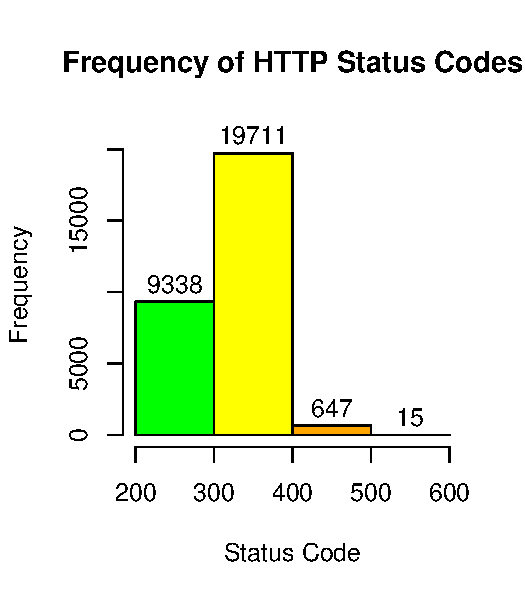
\includegraphics{stats/http_status_codes.pdf}
%    \caption{Frequency of HTTP status codes in histogram by sequential category.
%}
%\end{figure}



\bibliographystyle{plain}
\bibliography{../../cs751}

\end{document}
